In this chapter experiments with real servos will be conducted in order to, firstly, tune the parameters of the simulation (servo's characteristics) and, secondly, verify that the simulation correctly predicts the behaviour of a real-life configuration.

\section{Experimental set-up}
The set-up is explained on \cref{fig:exp_setup}. In later experiments a camera will be used to film the motion of the servos and compare it to the results of the simulation that is supposed to predict it.

\begin{figure}[htp]
\center
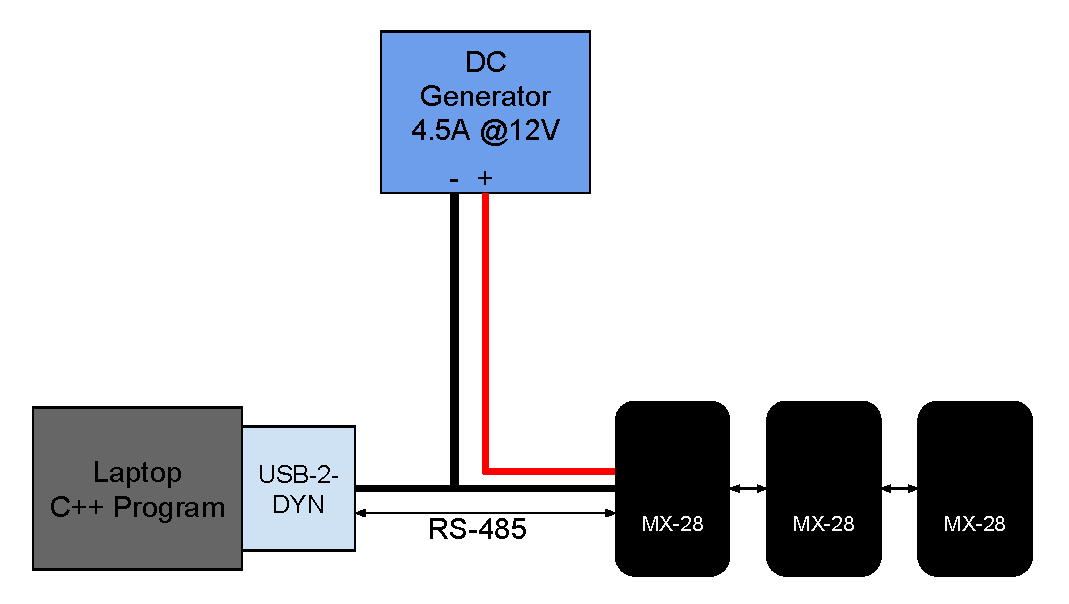
\includegraphics[width=0.6\textwidth]{figures/exp_setup}
\caption[Experimental setup]{Experimental setup : The MX-28 servos are powered by a DC generator and controlled by a laptop equipped with a USB2DYNAMIXEL(USB-2-DYN) device. It converts an USB port into a serial port.}
\label{fig:exp_setup}
\end{figure}

\section{Experiment 1}
The purpose of the first experiment is to test the torque : to that end, a frame is fixed onto a single servo and weighted. The setup is represented on \cref{fig:exp1}.

\begin{figure}[htp]
\center
    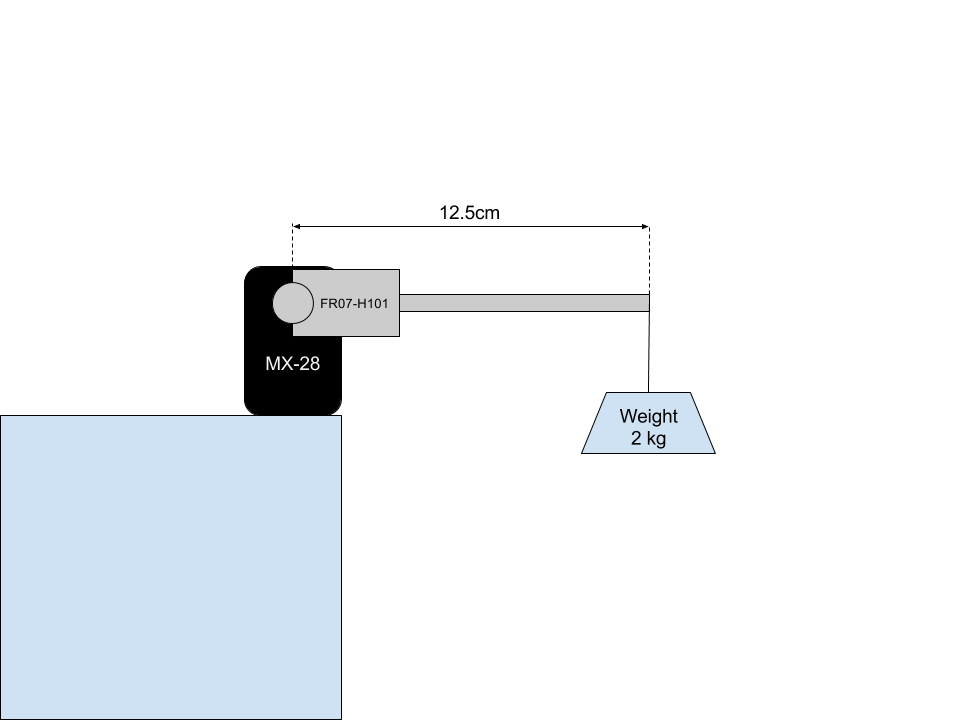
\includegraphics[width = 0.5\textwidth]{figures/exp1}
    \caption[Experimental setup for torque testing]{Experimental setup for torque testing. A weight $w$ of is suspended at a distance $d$ from the servo, resulting in a applied torque of $w \times g \times d$. The goal consists in finding the weight $w$ for which the servo is unable to lift the arm.}
    \label{fig:exp1}
\end{figure}

In our case, $d$ was equal to $22.5cm$ and we could reach a weight $w$ of $740g$ at $1.84V$. This equals to a torque of $1.64Ncm$. The complete results are listed in \cref{table:exp1_results}.
\begin{table}[htp]
\center
\begin{tabularx}{\textwidth}{@{}l X X X @{}}
\toprule
& \textbf{Stall torque @11.1V $[N.m]$} & \textbf{Stall torque @12V $[N.m]$} & \textbf{Stall torque @14.8V $[N.m]$}\\ 
\midrule
\textbf{Theoretical} & 2.1 & 2.5 & 3.1\\ 
\textbf{Experimental} &  &  & 1.64\\ 
\bottomrule
\end{tabularx}
\caption[Results of experiment 1]{Experimental stall torques at different tested voltages. Theoretical values taken from \cite{mx_28_manual}}.
\label{table:exp1_results}
\end{table}

\section{Experiment 2}


\section{Conclusion}